\documentclass{article}
\usepackage[UTF8]{ctex}
\usepackage{geometry}
\usepackage{natbib}
\geometry{left=3.18cm,right=3.18cm,top=2.54cm,bottom=2.54cm}
\usepackage{graphicx}
\pagestyle{plain}	
\usepackage{setspace}
\usepackage{caption}
\usepackage{datetime} %日期
% \usepackage{url}
\usepackage[colorlinks,linkcolor=black]{hyperref}
\renewcommand{\today}{\number\year 年 \number\month 月 \number\day 日}
\renewcommand{\captionlabelfont}{\small}
\renewcommand{\captionfont}{\small}
\begin{document}

\begin{figure}
    \centering
    
\includegraphics[width=8cm]{upc.png}

    \label{figupc}
\end{figure}

	\begin{center}
		\quad \\
		\quad \\
		\heiti \fontsize{45}{17} \quad \quad \quad 
		\vskip 1.5cm
		\heiti \zihao{2} 《信息技术前沿讲座》课程总结报告
	\end{center}
	\vskip 2.0cm
		
	\begin{quotation}
% 	\begin{center}
		\doublespacing
		
        \zihao{4}\par\setlength\parindent{7em}
		\quad 

		学生姓名:\underline{\qquad  田康康 \qquad \qquad}

		学\hspace{0.61cm} 号:\underline{\qquad 1606050112\qquad}
		
		专业班级:\underline{\qquad 计科1702 \qquad  }
		
        学\hspace{0.61cm} 院:\underline{计算机科学与技术学院}
% 	\end{center}
		\vskip 2cm
		\centering
		\begin{table}[h]
            \centering 
            \zihao{4}
            \begin{tabular}{|c|c|c|c|c|c|c|}
            % 这里的rl 与表格对应可以看到,姓名是r,右对齐的;学号是l,左对齐的;若想居中,使用c关键字。
                \hline
                课程认识 & 问题思 考 & 格式规范  & IT工具  & Latex附加  & 总分 & 评阅教师 \\
                30\% & 30\% & 20\% & 20\% & 10\% &  &  \\
                \hline
                 & & & & & &\\
                & & & & & &\\
                \hline
            \end{tabular}
        \end{table}
		\vskip 2cm
		\today
	\end{quotation}

\thispagestyle{empty}
\newpage
\setcounter{page}{1}
% 在这之前是封面,在这之后是正文
\section{引言}
信息技术(Information Technology,缩写:IT)也称信息和通信技术(Information and Communications Technology,ICT),是主要用于管理和处理信息所采用的各种技术总称,主要是应用计算机科学和通信技术来设计、开发、安装和部署信息系统及应用软件。依照存储和处理信息的不同,可以将信息技术的发展分为几个不同的阶段:前机械时期(3000 BC – 1450 AD)、机械时期(1450–1840)、机电时期(1840–1940)及电子时期(1940–现时)
\section{百年未有之大变局}
全面深刻认识“百年未有之大变局\citep{libin}”。\par
首先,“变”在何处?百年未有之大变局,变就变在前所未有、百年罕遇,变就变在立破并举、涤旧生新。这个大变局,概括起来说,就是当前国际格局和国际体系正在发生深刻调整,全球治理体系正在发生深刻变革,国际力量对比正在发生近代以来最具革命性的变化。即世界经济重心正在加快“自西向东”位移;新一轮科技革命和产业变革正在重塑世界;新兴市场国家和发展中国家国际影响力不断增强,国际力量对比更趋均衡;全球治理的话语权越来越向发展中国家倾斜,全球治理体系越来越向着更加公正合理的方向发展;世界文明多样性更加彰显,世界各国开放包容、多元互鉴成为主基调。\par
其次,“道”向何方?大变局的演进趋势,必然反映人类文明和平发展的大潮流大趋向。这个大变局,是从事实上“一家独大”的单极世界向协同共治的多极世界的重大转变;是现代化发展路径从一元走向多元的重大转变;是从社会主义遭遇严重挫折向科学社会主义在21世纪焕发勃勃生机的重大转变。当然也还要清醒认识到,世界格局的演变是一个由量变到质变的渐进过程。世界力量结构尚未发生根本性变化,美国等西方国家仍在经济、科技、军事等方面占据优势地位,资本主义制度仍然具有顽强的生命力,资本主义与社会主义两种制度、两种道路的斗争也将是漫长的、持久的。
\section{信息技术革命之人工智能}
新一代的信息技术革命中较早展露锋芒的就是人工智能\citep{poole1998computational}了。\par
人工智能亦称智械、机器智能,指由人制造出来的机器所表现出来的智能。关于什么是「智能」,较有争议性。这涉及到其它诸如意识、自我、心灵,包括无意识的精神等等问题。人唯一了解的智能是人本身的智能,这是普遍认同的观点。但是我们对我们自身智能的理解都非常有限,对构成人的智能必要元素的了解也很有限,所以就很难定义什么是「人工」制造的「智能」了。因此人工智能的研究往往涉及对人智能本身的研究。其它关于动物或其它人造系统的智能也普遍被认为是人工智能相关的研究课题。

人工智慧目前在计算机领域内,得到了愈加广泛的发挥。并在机器人、经济政治决策、控制系统、仿真系统中得到应用。\par
我现在正在参与“基于暗通道先验的图像去雾”的大创项目便使用了人工智能的相关研究方法,
本来我们的技术栈只使用了opencv、numpy等基础库,但是经过几个版本的迭代后发现使用卷积神经网络的单张图像去雾AOD-Net\citep{aod}算法效果更好,而且实现简单。我们最初使用的去雾算法
是基于物理模型的复原方法,这种方法通过研究大气悬浮颗粒对光的散射作用, 建立大气散射模型,了解图像退化的物理机理, 并复原出未降质前的图像。现在对暗通道先验的图像去雾的研究都是基于
何凯明博士的《Single image haze removal using dark channel prior》\citep{dehaze}。这种算法的原理是在绝大多数非天空的局部区域里,某一些像素总会有至少一个颜色通道有很低的值。
换言之,该区域光强度的最小值是个很小的数,这就是暗通道。\par
我们给暗通道一个数学定义,对于任意的输入图像J,其暗通道可以用下式表达:
\begin{equation}
J^{dark}\left ( x \right )=\min_{c\in\left \{ r,g,b \right \}\;\;y\in\Omega \left ( x \right )}\left ( min(J^{c}(y)) \right )
\end{equation}\par
众所周知,雾天中的拍摄的图片,在雾度比较高的地方成像效果较差,颜色较暗,这就是该算法需要识别并处理的区域。
知道了什么是暗通道之后,还需要雾图形成模型:
\begin{equation}
    I\left ( x \right )=J\left ( x \right )t\left ( x \right )+A\left ( 1-t\left ( x \right ) \right )    
\end{equation}\par
$J\left ( x \right )$即是我们需要求得的目标图像。经过一些数学变换后即可得变换公式,这里就不赘述:
\begin{equation}
    J\left ( x \right )=\frac{I\left ( x \right )-A}{max(t\left ( x \right ),t_{0})}+A
\end{equation}\par
这种算法有一个很大的缺点,该算法和以前的技术都是采用构建物理模型与各种复杂的图像统计假设来对图像进行去雾,比如“颜色衰减”模型,场景深度的线性模型,非局部先验的算法等,
而这对于单幅图像来说并没有包含这么多的准确信息,都是通过各种假设来获取到的相关参数,极不准确,所以去雾效果很难令人满意。
所以我们选择了其他的方向,我们的预期便是从单幅图像中直接构建出足够准确的传输矩阵,随着近年卷积神经网络的火热,
我们尝试性地构建了一种可训练的模型来估计一个有雾图像的传输矩阵,使用NYU等经典数据集生成大量的有雾、无雾的对比图对模型进行训练,然后再通过深度学习进行细分,获取足够清晰的去雾图像。\par
经过改进后的算法非常简单,使用了五层卷积神经网络,而且经过大数据集训练而得的模型通用性极佳,对单张图像去雾效果很好。\par
\begin{figure}[ht]
\centering
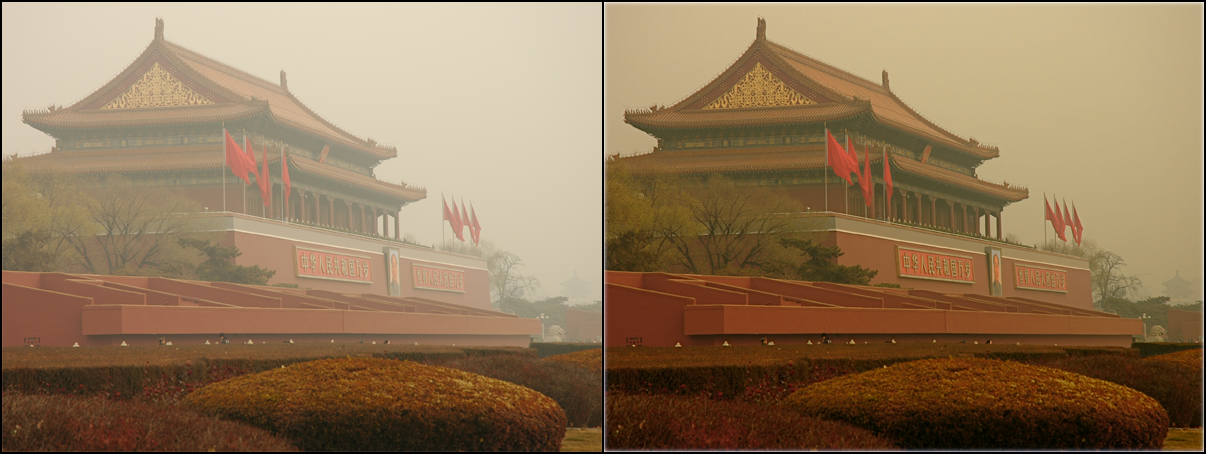
\includegraphics[scale=0.3]{dehaze1.png}
\caption{经典的天安门图像去雾对比}
\label{fig:label}
\end{figure}



% {\bf 注意,仅仅是引用的样例}\par
% \begin{figure}[ht]
% \centering
% 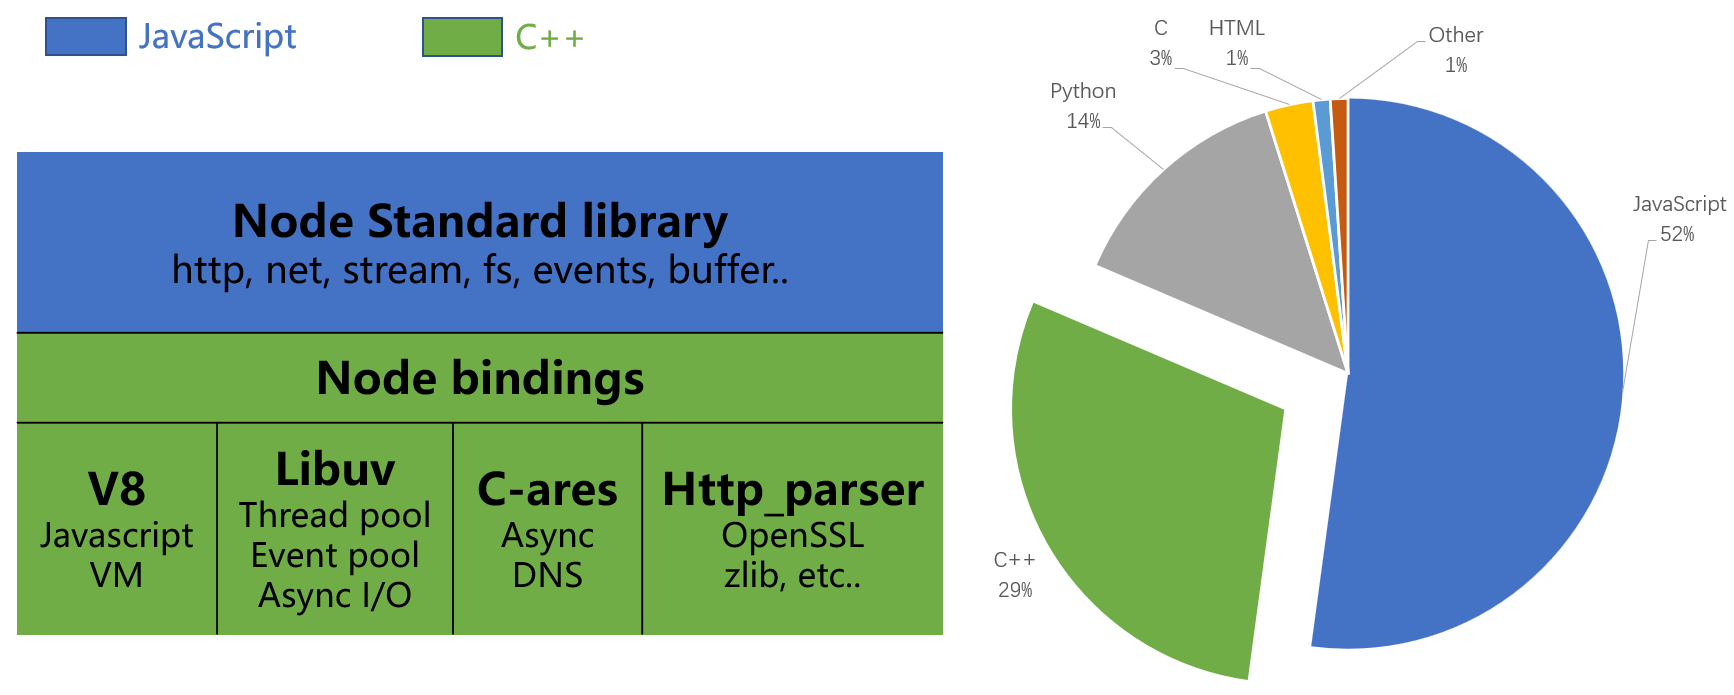
\includegraphics[scale=0.15]{nodecode.png}
% \caption{Node.Js源码概览}
% \label{fig:label}
% \end{figure}
\section{对服务端渲染的进一步思考}
在课程中的分组演讲中,我介绍的是“服务端渲染”,要想理解服务端渲染,首先要清楚一个渲染的概念:渲染即是数据与模版组装成 HTML 。为了更好的理解服务端渲染,我们可以将服务端渲染与客户端渲染对比着来看。\par
客户端渲染就是前端做视图和交互,后端只提供接口数据,前端通过 Ajax 向服务端请求数据,获取到数据后通过 JS 生成 DOM 插入 HTML 页面,最终渲染给用户。页面代码在浏览器源代码中看不到。\par
服务端渲染则是服务端在返回 HTML 之前,在特定的区域,符号里用数据填充生成 HTML ,再发送给客户端HTML,客户端解析HTML最终渲染出页面给用户,页面代码在浏览器源代码中看得到。\par
本质上两种渲染都是一样的,都是进行的字符串拼接生成HTML,两者的差别最终体现在时间消耗以及性能消耗上。客户端在不同网络环境下进行数据请求,客户端需要经历从js加载完成到数据请求再到页面渲染这个时间段。导致了大量时间的消耗以及浏览器性能的消耗。而服务端在内网请求,数据响应快,不需要等待js代码加载,可以先请求数据再渲染可视部分然后返回给客户端,客户端再做二次渲染,这样大部分消耗的是服务端的性能。客户端页面响应时间也更快。
这就可以解释为什么要使用服务端渲染。

与传统 SPA (单页应用程序 (Single-Page Application\citep{mikowski2013single})) 相比,服务器端渲染 (SSR) 的优势主要在于:
\begin{itemize}
    \item 更好的 SEO ,由于搜索引擎爬虫抓取工具可以直接查看完全渲染的页面。\par
    截至目前,Google 和 Bing 可以很好对同步 JavaScript 应用程序进行索引。在这里,同步是关键。如果应用程序初始展示 loading 菊花图,然后通过 Ajax 获取内容,抓取工具并不会等待异步完成后再行抓取页面内容。也就是说,如果 SEO 对站点至关重要,而页面又是异步获取内容,则可能需要服务器端渲染(SSR)解决此问题。
    \item 更快的内容到达时间,特别是对于缓慢的网络情况或运行缓慢的设备。\par
    无需等待所有的 JavaScript 都完成下载并执行,才显示服务器渲染的标记,所以用户将会更快速地看到完整渲染的页面。通常可以产生更好的用户体验,并且对于那些「内容到达时间(time-to-content) 与转化率直接相关」的应用程序而言,服务器端渲染 (SSR) 至关重要。
\end{itemize}
使用服务器端渲染时还需要有一些权衡之处:
\begin{itemize}
    \item 开发条件所限。\par
    浏览器特定的代码,只能在某些生命周期钩子函数中使用;一些外部扩展库可能需要特殊处理,才能在服务器渲染应用程序中运行。
    \item 涉及构建设置和部署的更多要求。\par
    与可以部署在任何静态文件服务器上的完全静态单页面应用程序不同,服务器渲染应用程序,需要处于 Node.js server 运行环境。
    \item 更多的服务器端负载。\par
    在 Node.js 中渲染完整的应用程序,显然会比仅仅提供静态文件的 server 更加大量占用 CPU 资源 (CPU 密集),因此如果在高流量环境下使用,需要准备相应的服务器负载,并明智地采用缓存策略。\par
\end{itemize}\par
还有一种解决方案就是使用同构:同构来源于一个数学概念,在数学中研究同构的主要目的是为了把数学理论应用于不同的领域。如果两个结构是同构的,那么其上的对象会有相似的属性和操作,对某个结构成立的命题在另一个结构上也就成立。因此,如果在某个数学领域发现了一个对象结构同构于某个结构,且对于该结构已经证明了很多定理,那么这些定理马上就可以应用到该领域。\par
同构开发在大前端中指的是使用相同的代码支持同时运行于服务端和客户端。区别于之前的 JSP/ASP 以及 template + data => HTML + 前端 JQuery 获取 DOM 绑定事件的服务端渲染方式,目前 Next.js/Nuxt.js 的同构渲染指的是组件可以在服务端运行,生成 HTML,再由客户端 Vue/React 接管从服务端吐出的 HTML,使其变为由客户端 Vue/React 管理的动态 DOM 的生成过程。\par
真正的同构即 CSR 和 SSR 写法一致,未来不再区分概念,比如在 ServerLess 里, API 和渲染都是函数。\par
总结上述,我认为同构在未来服务器性能得到大幅提升之后会越来越被开发团队所接受,没有 SSR 与 CSR 之分。



% 这里是简单列表的样例:(如果需要标号自定义或者自动标记数字序号,请自行搜索语法)
% \begin{itemize}
%     \item 简单的列表结构 
%     \item 如这里所示
%     \item 此处仅为样例
%     \item 按需修改和使用
% \end{itemize}


\section{总结}
写本报告大约用了一天的时间,大多时间是在查阅资料、重读PPT,加深自己对计算科学的理解,大部分的总结其实都写在上述文字里。我觉得查阅资料和重读PPT的过程才是收获最多的,读了很多文献、整理了自己的知识链,收获很多。\par
我们应该认识到高校开设的任何一学科都有其滞后性,在我们掌握了一门新技术同时会有更新的技术产生。而我们这一专业更为严重,更为突出,也许在校期间学习的东西在毕业后已经不适合用了。正如我们现在学习的程序语言,也许在走出校门后又会出现新的语言。所以说,我们要学好这一学科的知识,更需要创新,提高自学能力和接受新事物的能力。我们这一学科本来就是走在时代前沿的一门学科,更需要紧跟时代的步伐。


\newpage
\section{附录}
\begin{itemize}
    \item Github\par
    个人主页
    \url{https://github.com/kngkngtian}\par
    报告仓库
    \url{https://github.com/kngkngtian/Reports}
    \begin{figure}[ht]
        \centering
        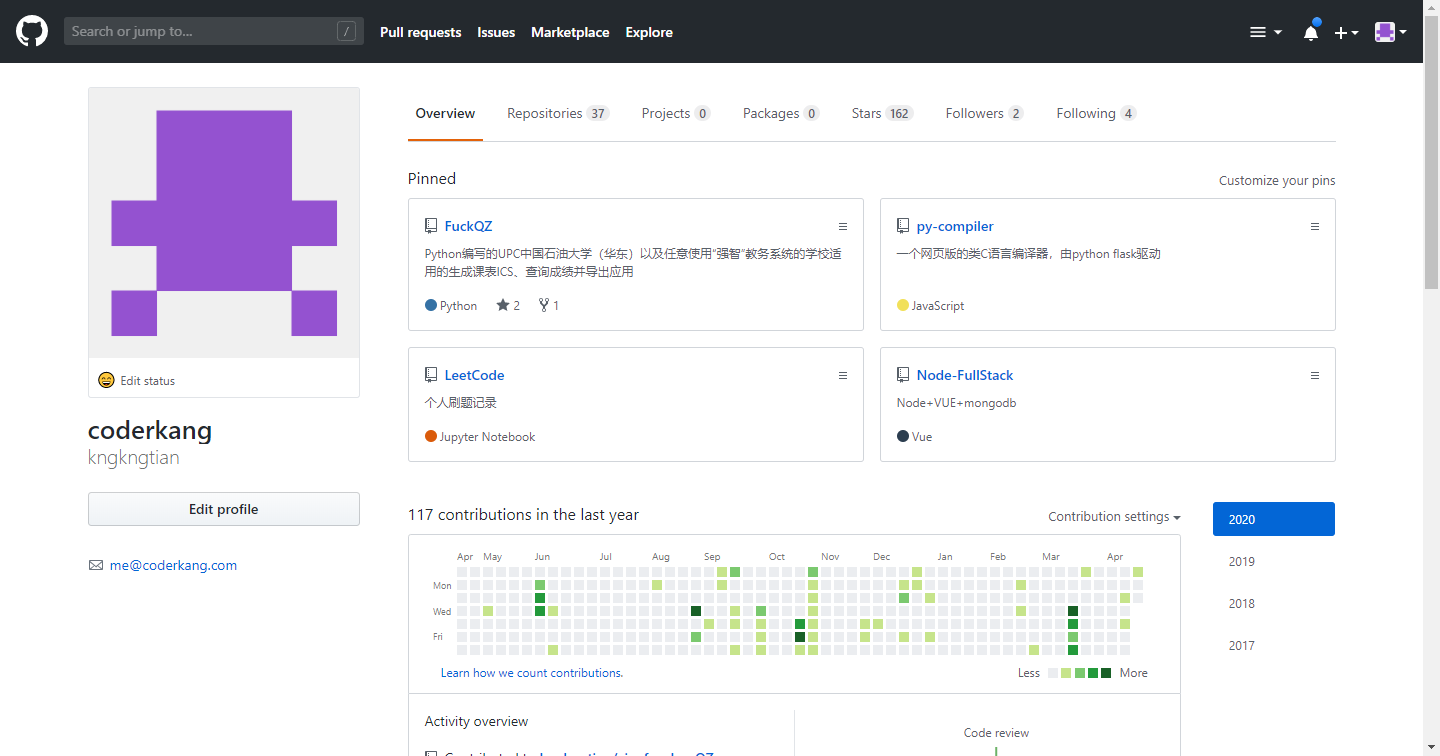
\includegraphics[scale=0.1]{github.png}
        \caption{Github个人主页}
        \label{fig:label}
        \end{figure}
    \newpage
    \item 观察者、学习强国、哔哩哔哩
    \begin{figure}[ht]
        \centering
        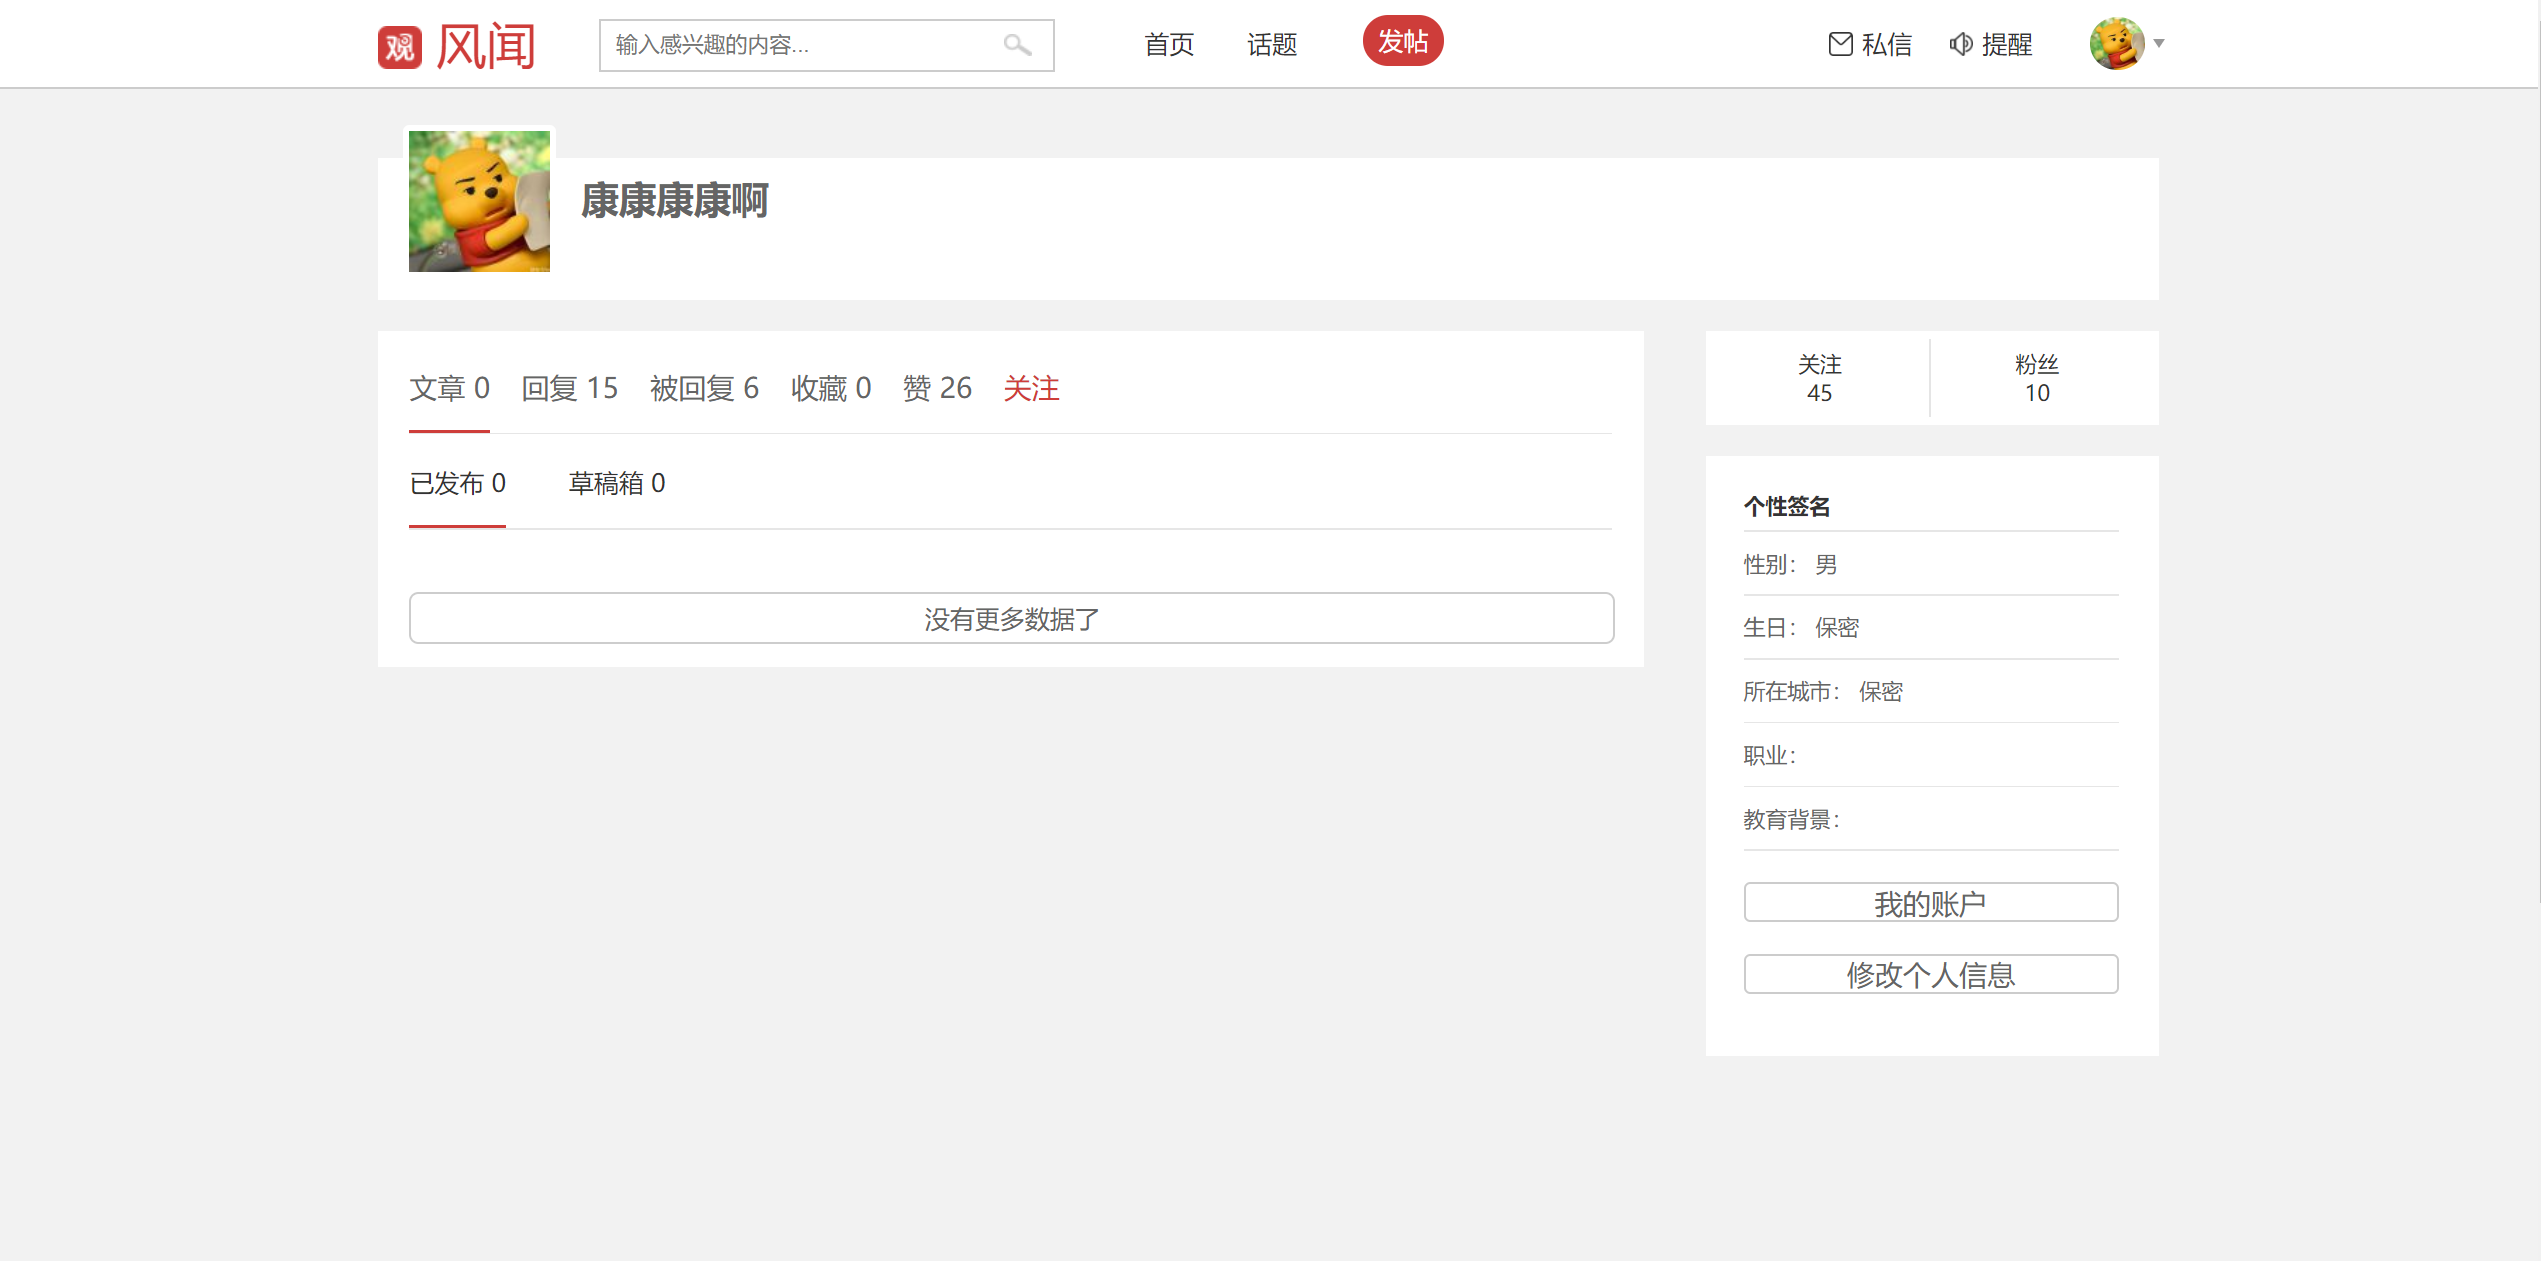
\includegraphics[scale=0.1]{gcz.png}
        \caption{观察者网}
        \label{fig:label}
        \end{figure}
    \begin{figure}[ht]
        \centering
        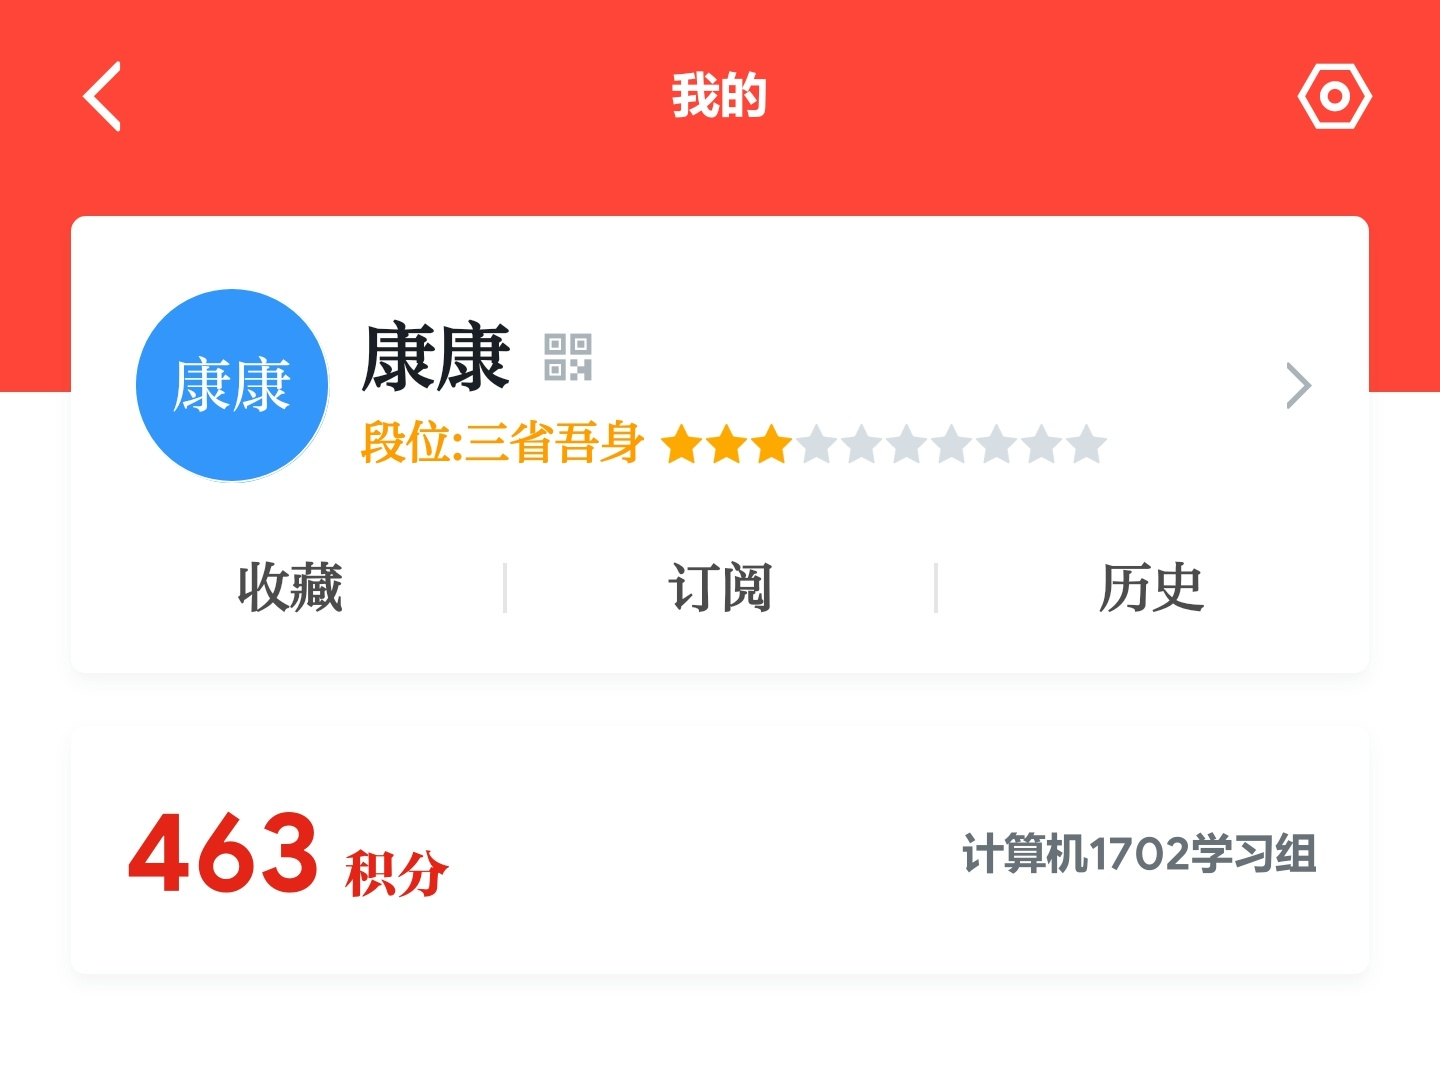
\includegraphics[scale=0.11]{xxqg.jpg}
        \caption{学习强国}
        \label{fig:label}
        \end{figure}
    \begin{figure}[ht]
        \centering
        
\includegraphics[scale=0.11]{bilibili.jpg}
        \caption{Bilibili}
        \label{fig:label}
        \end{figure}
    \newpage
    \item CSDN、博客园\par
    CSDN个人主页
    \url{https://blog.csdn.net/coderkang}\par
    \begin{figure}[ht]
        \centering
        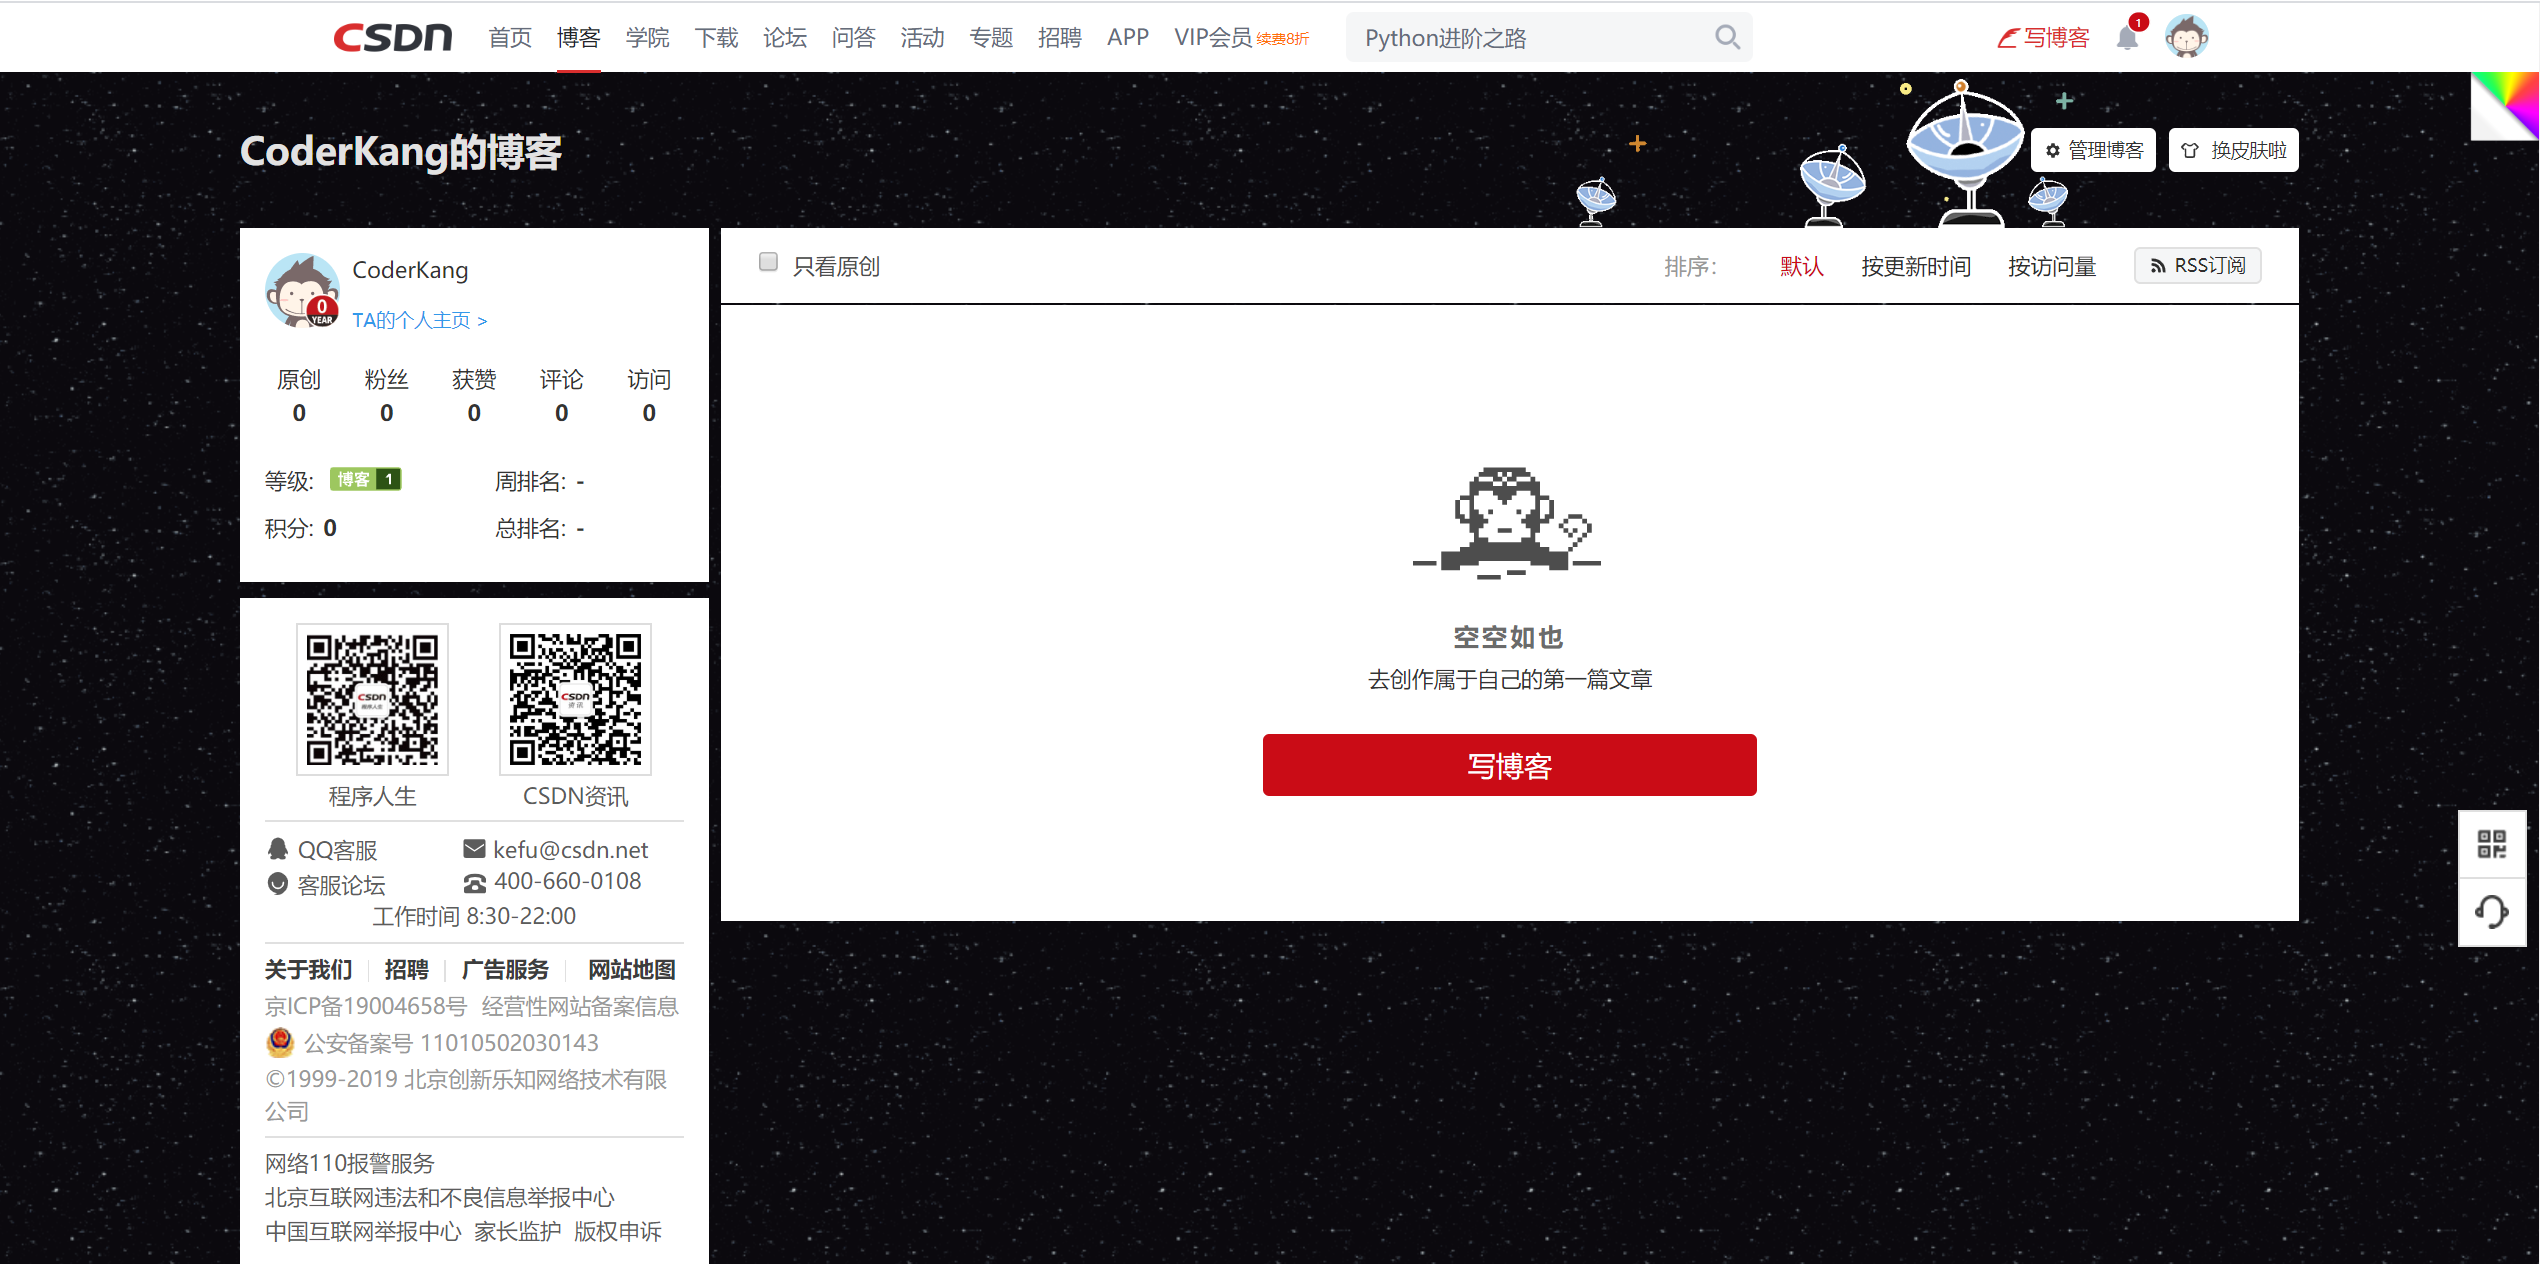
\includegraphics[scale=0.1]{csdn.png}
        \caption{CSDN}
        \label{fig:label}
        \end{figure}
    博客园个人主页
    \url{https://www.cnblogs.com/coderkang/}\par
    \begin{figure}[ht]
        \centering
        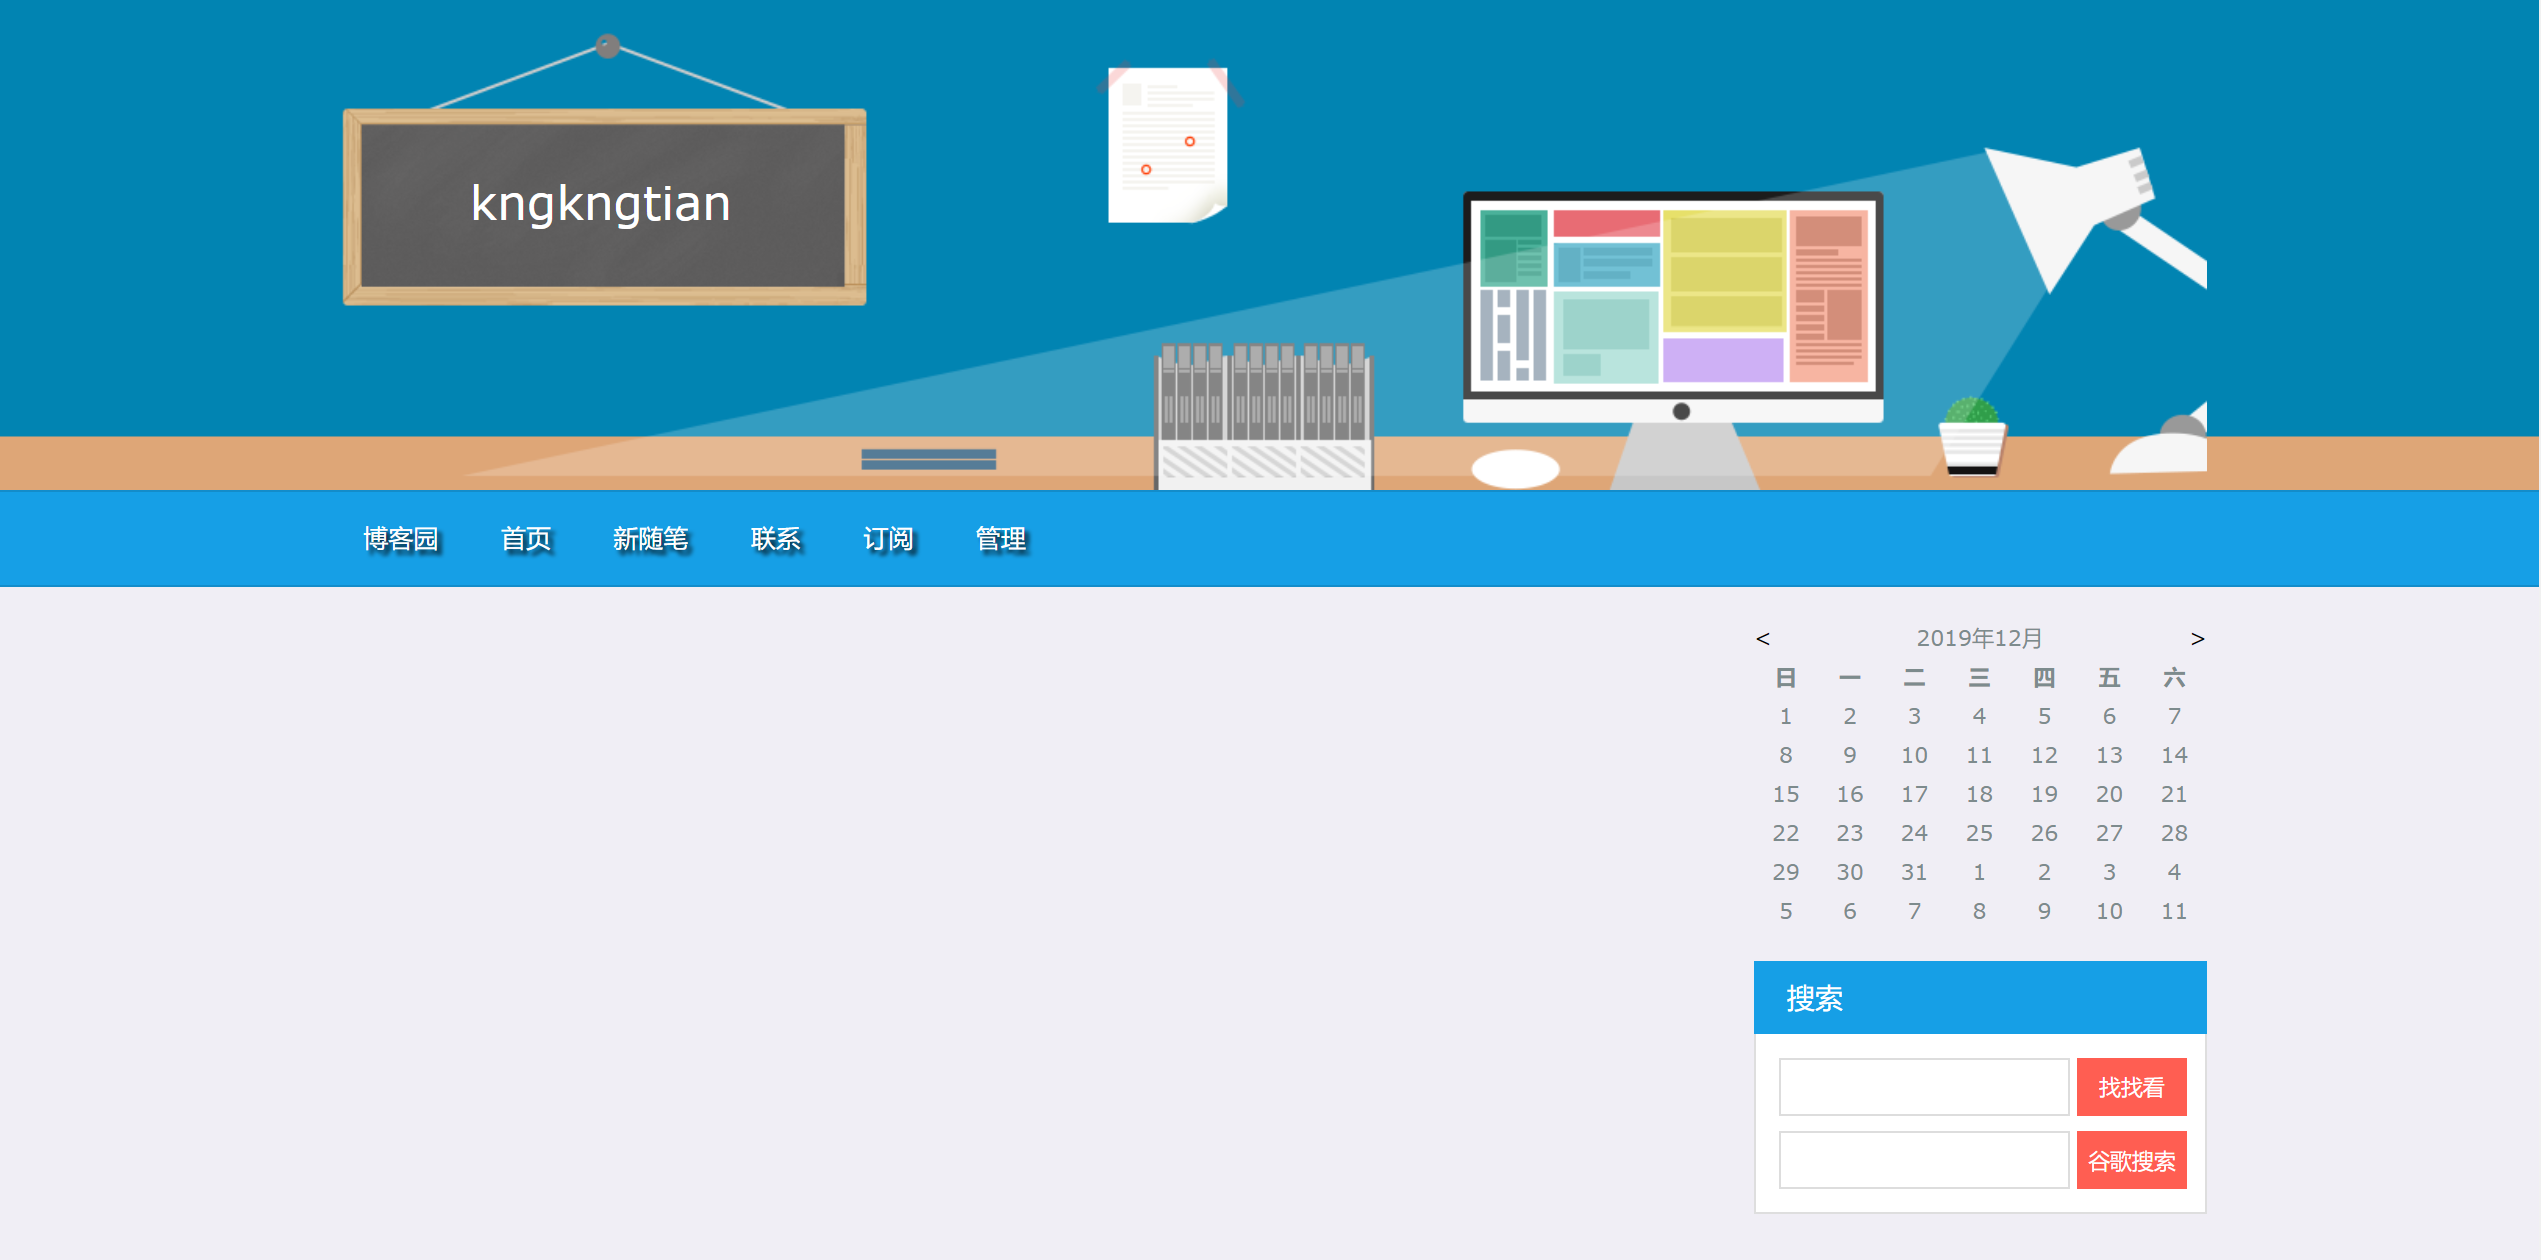
\includegraphics[scale=0.1]{cnblog.png}
        \caption{博客园}
        \label{fig:label}
        \end{figure}
    \item 小木虫\par
    个人网址
    \url{http://muchong.com/bbs/space.php?uid=20339032}\par
    \begin{figure}[ht]
        \centering
        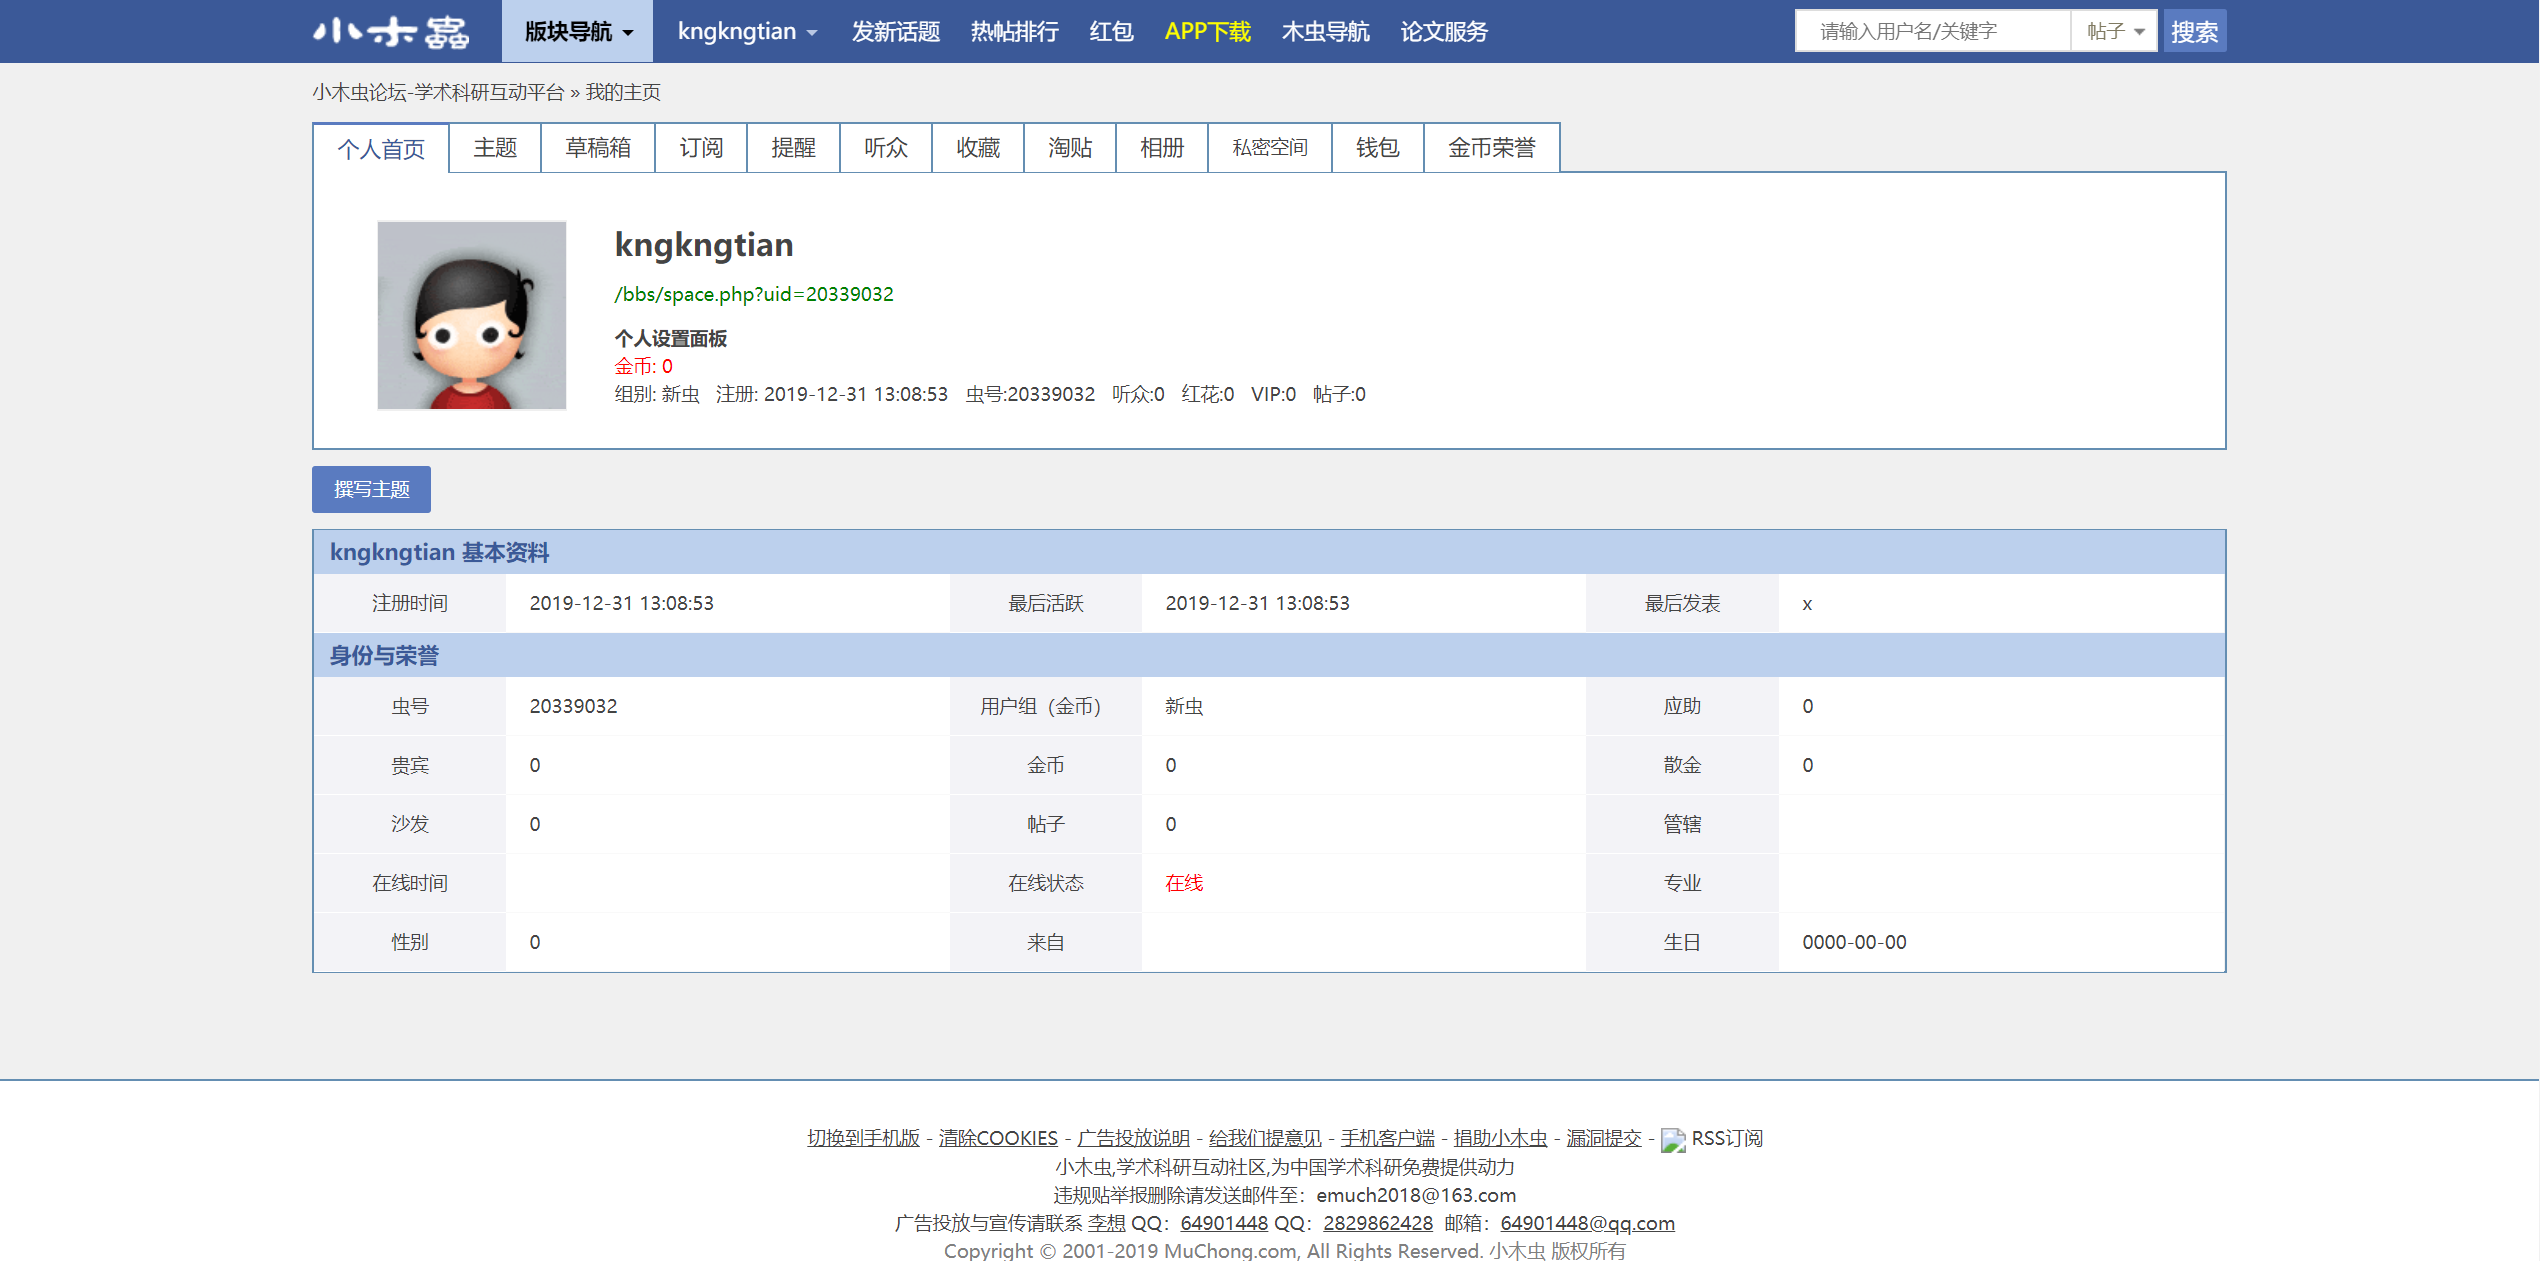
\includegraphics[scale=0.1]{xmc.png}
        \caption{小木虫}
        \label{fig:label}
        \end{figure}
\end{itemize}


\hspace*{\fill} \\

% {\bf 注意,参考文献至少五篇,其中至少两篇为英文文献,参考文献必须在正文中有引用。}
% \bibliographystyle{plain}
\bibliographystyle{unsrt}
\bibliography{references}


\end{document}
